\section{Понятие абстрактного цифрового автомата}

\subsection{Постановка задачи}

Привести обобщенную структурную схему автомата Мили.
Пояснить векторное представление абстрактного автомата:
описание входов/выходов, начального состояния, функций переходов и функций выходов, состояний памяти.
Пояснить способ табличного представления работы автомата и в виде графа автомата.

\subsection{Обобщенная структурная схема автомата Мили}

В обобщенном виде автомат представляет собой устройство с одним входом, на который подается набор логических сигналов, одним выходом,
на котором формируется набор логических сигналов, и блоком памяти, который хранит текущее состояние автомата.
Состояние памяти определяется функцией, зависящей от входного сигнала и предыдущего состояния памяти.
В автомате Мили выходной сигнал определяется функцией, зависящей не только от состояния памяти, но и от входного сигнала автомата.
На рисунке \ref{fig:task4:scheme} представлена обобщенная структура автомата Мили.

\begin{figure}[h!]
    \centering
    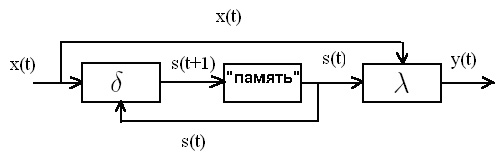
\includegraphics[scale=0.7]{S4IM1.jpg}
    \caption{Обобщенная структурная схема автомата Мили}
    \label{fig:task4:scheme}
\end{figure}

\subsection{Векторное представление абстрактного автомата}

Векторное представление абстрактного автомата имеет вид:
%
\begin{equation*}
    S = (A, Z, W, \delta, \lambda)
\end{equation*}

\begin{explanation}
    \item[где] $A$ - множество состояний памяти автомата;
    \item $Z$ - множество входных сигналов;
    \item $W$ - множество выходных сигналов;
    \item $\delta: A \times Z \rightarrow A$ - функция переходов, определяющая внутреннее состояние памяти автомата;
    \item $\lambda$ - функция выходов, определяющая выходной сигнал автомата.
\end{explanation}

\pagebreak

Абстрактный автомат с некоторым выделенным состоянием памяти $a_0$ называется инициальным автоматом.
Таким образом, один неинициальный автомат с n состояниями задает семейство из n различных инициальных автоматов \cite{automats}.
Если начальное состояние не указано, то поведение автомата всегда недетерменированно, выходное слово зависит от начального состояния,
поэтому полное детерменированное векторное представление абстрактного автомата имеет вид:
%
\begin{equation*}
    S = (A, Z, W, \delta, \lambda, a_0)
\end{equation*}

В зависимости от функции выходов $\lambda$ выделяют два класса автоматов: 
автомат Мура - выходной сигнал которого не зависит от входного сигнала $(\lambda: A \rightarrow W)$
и автомат Мили, выходной сигнал которого зависит как от внутреннего состояния, так и от состояния входа $(\lambda: A \times Z \rightarrow W)$.

\subsection{Табличное представление работы автомата}

Работу автомата можно представить в табличном виде. Для этого составляются таблицы функции перехода $\delta$ и функции выхода $\lambda$.
Строки таблиц отмечают входными символами (элементами множества Z), а столбцы - состояниями памяти (элементами множества A).

В таблице, задающей функцию переходов $\delta$ на пересечении строки $z_i(t)$ и столбца $a_j(t)$ 
ставится состояние $a_k(t+1) = \delta(z_i(t), a_i(t))$:

\begin{table}[h!]
    \caption{Таблица функции переходов $\delta$}
    \begin{tabular}{| >{\centering}m{0.05\textwidth} 
                    | >{\centering}m{0.05\textwidth} 
                    | >{\centering}m{0.05\textwidth} 
                    | >{\centering}m{0.05\textwidth} 
                    | >{\centering\arraybackslash}m{0.05\textwidth}|} 
        \hline $\delta$  &  $a_1$  &  $a_2$  &  $a_3$  &  $a_4$ \\
        \hline  $z_1$    &  $a_2$  &  $a_2$  &    -    &  $a_4$ \\
        \hline  $z_2$    &  $a_4$  &    -    &  $a_1$  &  $a_3$ \\        
        \hline  $z_3$    &  $a_3$  &  $a_3$  &  $a_4$  &    -   \\
        \hline
    \end{tabular}
    \label{tab:task4:table1}
\end{table}

В таблице, задающей функцию выходов $\lambda$ на пересечении строки $z_i(t)$ и столбца $a_j(t)$
ставится состояние $w_k(t) = \lambda(z_i(t), a_i(t))$:

\begin{table}[h!]
    \caption{Таблица функции выходов $\lambda$}
    \begin{tabular}{| >{\centering}m{0.05\textwidth} 
                    | >{\centering}m{0.05\textwidth} 
                    | >{\centering}m{0.05\textwidth} 
                    | >{\centering}m{0.05\textwidth} 
                    | >{\centering\arraybackslash}m{0.05\textwidth}|} 
        \hline $\lambda$  &  $a_1$  &  $a_2$  &  $a_3$  &  $a_4$ \\
        \hline  $z_1$     &  $w_1$  &  $w_2$  &    -    &  $w_3$ \\
        \hline  $z_2$     &  $w_2$  &    -    &  $w_4$  &  $w_5$ \\        
        \hline  $z_3$     &  $w_3$  &  $w_1$  &  $w_3$  &    -   \\
        \hline
    \end{tabular}
    \label{tab:task4:table2}
\end{table}

Таблицы \ref{tab:task4:table1}, \ref{tab:task4:table2} задают 
функцию переходов $\delta$ и функцию выходного сигнала $\lambda$ для автомата c множеством состояний $|A| = 4$, 
множеством входных сигналов $|Z| = 3$
и множеством выходных сигналов $|W| = 5$.

\subsection{Представление работы автомата в виде графа}

Более наглядным описанием закона функционирования автомата является представление его в виде графа.
Граф автомата -- это ориентированный граф, вершины которого соответствуют состояниям, а дуги -- переходам между ними.

Дуга, направленная из вершины $a_i$ в вершину $a_j$ соответствует переходу из состояния $a_i$ в состояние $a_j$.
В начале дуги записывается входной символ $z_k$, влияющий на переход, а символ $w_k$ записывается на конце дуги (для автомата Мили)
или рядом с вершиной (для автомата Мура). 

На рисунке \ref{fig:task4:graph} приведен граф автомата Мили, соответствующий закону функционирования, 
описанному таблицами \ref{tab:task4:table1}, \ref{tab:task4:table2}.

\begin{figure}[h!]
    \centering
    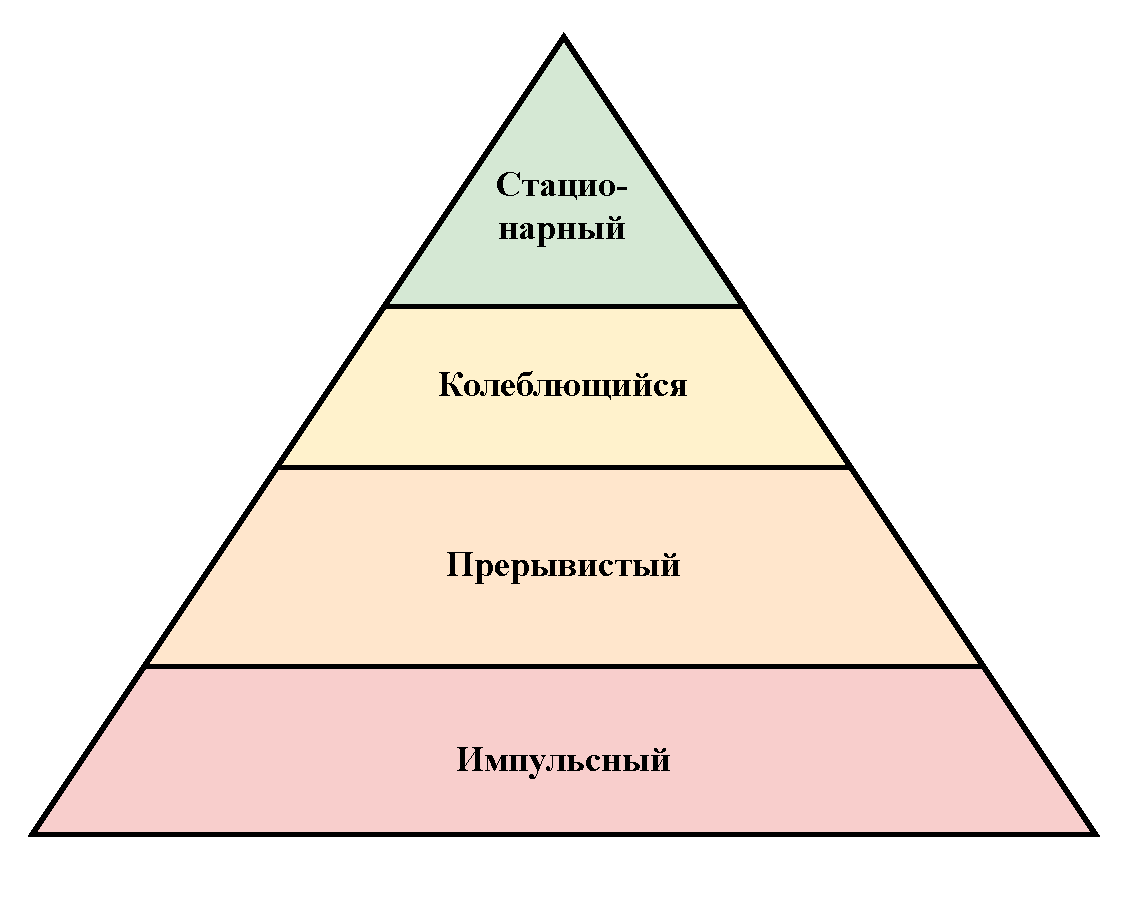
\includegraphics[scale=1.2]{S4IM2.pdf}
    \caption{Граф абстрактного автомата Мили}
    \label{fig:task4:graph}
\end{figure}